\section{Signal processing}
The space for improvement in the signal processing parts is very large.
Actually, you can consider any possible function that maps an audio sequence to an integer giving the predicted class. The only contextual constraint is that you must send somehow the acquired information wirelessly from the transmitter to the receiver. Then you also have to take into account the physical constraints imposed by your devices in terms of sampling, processing, memory, data rate and energy consumption. The priority when optimizing a working project is to identify the bottlenecks, i.e. the parts that are the most limiting the performances. Think about it before spending 3 weeks on something which would give negligible improvements at the end. To organize your reasoning, you can decompose the signal processing (without the authentication and packet creation aspects) in three main steps:

%%%%%%%%%%%%%%%%%%%%%%%%%%%%%%%%%%%%%%%%
\subsection{Feature vector shaping}
%%%%%%%%%%%%%%%%%%%%%%%%%%%%%%%%%%%%%%%%

\begin{figure}[H]
    \centering
    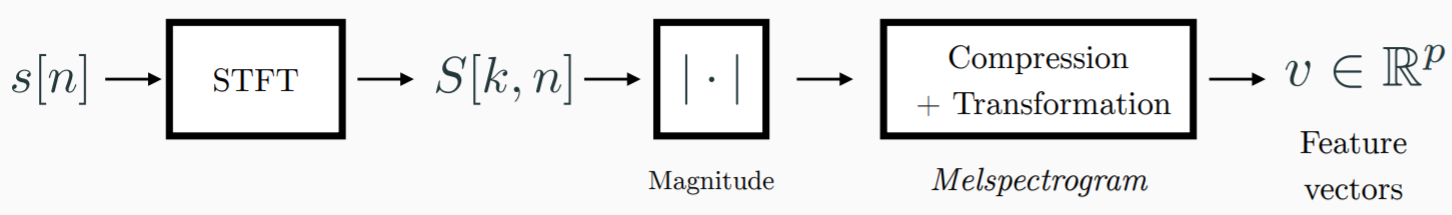
\includegraphics[width=14cm]{figs/scheme.PNG}
    \caption{Computation chain from temporal audio signal to feature vector.}
    \label{fig: fv}
\end{figure}
During the first semester, we provided you with a time-frequency representation that was compressed using the Hz$\rightarrow$mel transformation, as depicted in Figure \ref{fig: fv}. This choice is interesting because it yields intuitive observations and results for a human. To optimize this step, you can consider another block scheme. You could for instance choose another way of compressing the information than using Mels. Or you could keep a pure temporal representation and compress it another way.
However, this is not compulsory and we argue the current scheme in Figure \ref{fig: fv} is already efficient. \\
What can be done is to keep this scheme and play with its parameters. You can vary the window size and shape for the STFT. You can vary the number of mels. And mainly, these computations are all made in C code in a fixed-point representation. We voluntarily wrote non optimal code. \\
Finally, a way to save energy on your device is to avoid computing feature vectors when you think the currently acquired sound does not contain anything important. A first approach we can think of is an energy threshold, where we decide not to compute the feature vector if the sound is not loud enough.

To synthesize, some options are:
\begin{itemize}
    \item Change the feature vector computation scheme.
    \item Optimize this scheme by tuning its parameters and improving the
    fixed-point implementation.
    \item Imagine criteria for starting the computation of the feature vector.
\end{itemize}
%
%%%%%%%%%%%%%%%%%%%%%%%%%%%%%%%%%%%%%%%%
\subsection{Classification}
%%%%%%%%%%%%%%%%%%%%%%%%%%%%%%%%%%%%%%%%

\begin{figure}[H]
    \centering
    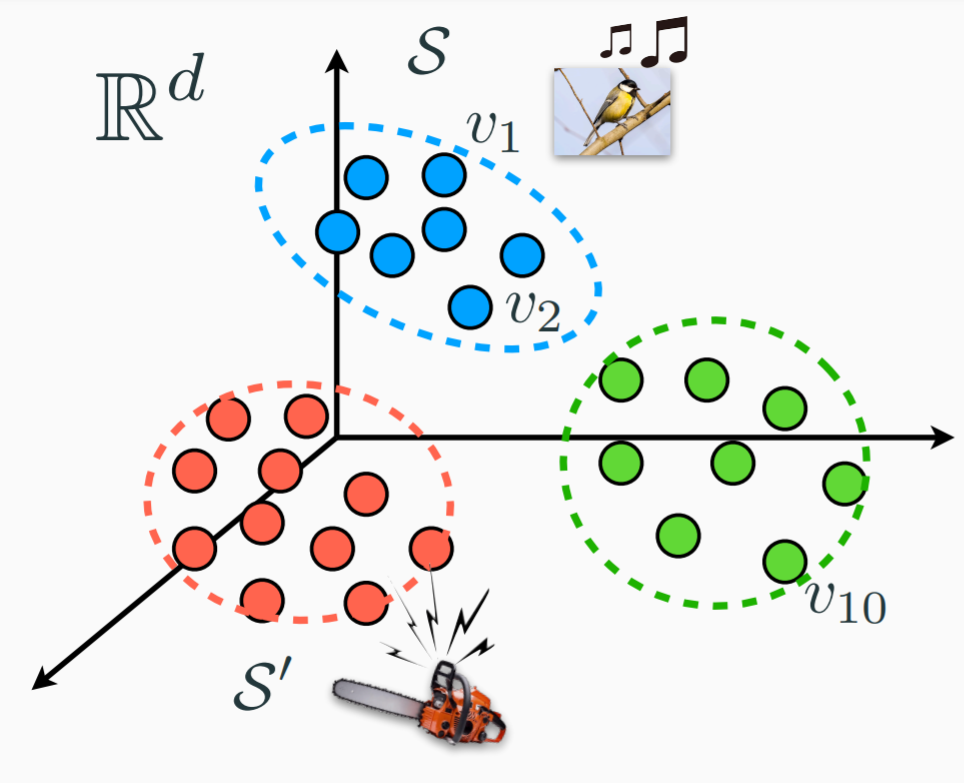
\includegraphics[width=8cm]{figs/classification.PNG}
    \caption{Classification principle.}
    \label{fig: classification}
\end{figure}
Once the feature vector computation process is fixed, the information contained in this feature vector has to be exploited at the receiver side for the classification, as shown in Figure \ref{fig: classification}. During the first semester, we already let you the possibility to play with different simple classifiers. The choice of the classifier is crucial and we advise you to test even more sophisticated ones to boost your perfomances. But remember to avoid overfitting! \\
You could consider the possibility to have a confidence metric on your predictions (remember that most classifiers provide first a probability of correct classification before to make a decision). This can be accompanied by a way to strenghten this confidence with the increasing amount of information provided by new features vectors. \\
Until now, you are classifying no matter what. There are situations where it is preferable not to output a prediction (i) the energy of the acquired sound is too low and you don't want to compute the feature vector on it (ii) your classifier outputs a probability vector balanced and no class is really highlighted. You are encouraged to manage these situations for the end of this project.


To synthesize, some options are:
\begin{itemize}
    \item Change the classifier.
    \item Add a confidence metric and exploit time to increase this confidence.
    \item Consider a threshold to output no class.
\end{itemize}

%%%%%%%%%%%%%%%%%%%%%%%%%%%%%%%%%%%%%%%%
\subsection{Training data}
%%%%%%%%%%%%%%%%%%%%%%%%%%%%%%%%%%%%%%%%

The way you train your classification model in this project is by using labelled (or training) data. This data is as important as the classifier choice. During the first semester, you trained your model with clean audio samples from the ESC-50 dataset, and discovered the possibility to augment this data by adding some transformations aiming to mimick real life perturbations. Now you master your devices and acquisition procedures, a better option is to create training data using your device. It implicitely takes the acquisition non idealities into account, and gives you the possibility to truly augment the data increasining the distance between the sound source and microphone, or adding background sound by yourself. \\
\\
Don't hesitate to discuss all your ideas with the TA's!
